\chapter{Accurate Soft Error Simulation Using Adaptive Partitioning} 

As technology continues to the scale down, the likelihood of a radiation induced error increases. This trend provides a need for accurate and efficient methods to calculate the soft error rate of a given circuit. Since it is expensive and time consuming to design and circuit and test at a later time, efficient tools that can accurately determine the error rate for a given netlist before fabrication can significantly reduce the design time. However, it has proven to be very difficult to characterize combinational circuits due to three pulse masking factors. The masking factors are as follows:

\begin{enumerate}
	\item Logical Masking: The pulse is removed due to the boolean inputs on the gate during pulse generation or a controlling value on an off-input during pulse propagation.
	
	\item Electrical Masking: The first order RLC effects within the gate cause the pulse to degrade and fully attenuate.
	
	\item Temporal Masking: The pulse arrives at a flip-flop but does not meet the set-up and hold time parameters. 
\end{enumerate}

Considering the above factors, all current soft error simulators consist of modeling a particle at a specific energy which is used in an equation to model the error pulse shape \cite{injeq}. Once the pulse is generated, it is propagated through the combinational logic to the output. It is then assumed that the output is connected to a flip-flop thus the set-up and hold times are considered. It has been shown in \cite{MARS_C,METSys} that concurrent estimation of all masking factors is required in order to ensure that the soft error rate is calculated accurately. However, due to limitations on simulation time and available memory, efficient and accurate consideration of all masking factors has proven to be a difficult and ongoing problem. 

There have been many approaches to improve the estimation of the three factors. First the existing approaches to the estimation of logical masking will be discussed. The most common method to calculate the logical masking effects is the use of a Monte Carlo based simulation which consists of randomly applying patterns as in \cite{Accurate_Masking,SERA,SEMM,PARAM_DESC,SETA_LA}. While this approach is very easy to implement, it suffers from accuracy and run time issues when the circuit has more than 30 inputs. In the case of large circuits, the simulator must resort to generating random input patterns which cover only a small subspace of the possible inputs. This implies that the error in logical masking estimation increases with the circuit size. 

To enhance on Monte Carlo based simulation, the authors in \cite{PTM} propose the use of probabilistic transfer matrices (PTM). This approach consists of representing the Boolean functions within a matrix in which Boolean operations can be applied. While being very accurate, the use of PTMs are non-ideal since they have high memory and simulation time costs that explode on small circuits. The authors in \cite{Han2014} propose an enhanced alternative to the PTM method which uses stochastic logic to calculate the signal probabilities for logical masking estimation. While their method is fast, it relies on the use of random input patterns that can limit the accuracy of the calculation.

Another common approach found in \cite{Chen2013,Li2016} uses the correlation coefficient method (CCM) proposed in \cite{Ercolani1989}. This method uses basic gate signal probability functions to determine the output. For example, the probability of an AND gate is given as $P(O) = P(A)P(B)$ where $P(O)$ is the output probability, $P(A)$ is the probability of input $A$ being "1" and $P(B)$ is the probability of inputs $B$ being "1". A drawback with using the basic probability functions is that they are unable to consider the correlations between signals. CCM improves on this by add a correlation factor to estimate the signal probability. While CCM does provide quick estimation of the logical masking effects with virtually no memory overhead, it can only estimate first order correlation. This implies that as the circuit gets larger, the accuracy of the method substantially decreases.

The last approach discussed in this section, which is of most concern in this paper, is the use of binary decision diagrams (BDDs). BDDs provide a very accurate way to determine the logical masking effects since they are a condensed canonical form of a Boolean function. The main problem with BDDs however, is that they scale exponentially with circuit size thus leading to the possibility of blow up on medium to large circuits. Despite this problem, there have been many proposed simulators that the use BDDs \cite{FASER,MARS_C,METSys}. The main advantage to the use of BDDs is that all input patterns can be considered concurrently thus allowing for exact calculation of logical masking probabilities.

To alleviate the inherent blow up problem, the authors in \cite{FASER} propose the use of partitioning. In their work, they show that the use of partitioning allows for much faster calculation of the soft error with no threat of blow up at a cost of accuracy. The authors in \cite{METSys} also investigate partitioning but do not give an in depth study on how partitioning effects the output error. In both approaches, the circuit is partitioned before simulation with each partition size being set to a predetermined value. This is problematic since the size may be much smaller or larger compared to the given time, processing power and memory. For this reason, this section proposes the use of an adaptive partitioning algorithm that scales the partition size based on the number of nodes. It is shown that the adaptive method allows for faster and more accurate estimation of the logical masking effect compared to the non adaptive approach.

In addition to the adaptive partitioning approach, the proposed simulator has the capability of considering multiple concurrent pulse strikes commonly referred to as multiple event transients (METs). The consideration of multiple strikes has become of greater concern due to the small feature size, leading to a lower critical charge for upset, and the closer placement of transistors \cite{Rossi2005}. These type of events can occur in two forms: single event multiple transient (SEMT) and multiple event multiple transient (MEMT). A SEMT is defined as the case where a single radiation particle upsets multiple transistors causing multiple transients pulses. A MEMT is defined as when multiple particles hit different circuit components simultaneously. While the probability of the SEMT vs the MEMT depends strongly on the radiation environment, methods developed for one type of error can easily be modified to consider the other. 

There are a few existing methods that include the consideration of multiple event errors. The authors in \cite{METSys} consider the correlation of METs however their method uses BDDs which tend to blow up. While they do investigate the use of partitioning, their method is only tested for small circuits using only a few concurrent pulses. An additional simulation tool used for MET analysis found in \cite{Fazeli2011} uses probabilistic functions. This approach has shown to be fast and efficient but is not suited for the use of complicated electrical masking methods. To improve on the existing methods, the simulator FAST\_MET (Fast and Accurate Simulation Tool for Multiple Event Transients) which uses BDDs to calculate the logical maksing effect in conjunction with the accurate pulse approximation tool proposed in Chapter \ref{ch2}. FAST\_SET improves on the method in \cite{METSys} by allowing for the integration of accurate electrical masking models and through the extensive use and evaluation of partitioning to avoid BDD blow up.    

\section{Preliminaries} \label{ch3:prelim}

A crucial aspect in the estimation of the logical masking effects is accurate creation of the Boolean functions. To ensure full consideration of the logical masking effects, Boolean functions must be created to evaluate the circuit inputs for pulse generation and the off-inputs for pulse propagation. First the method to generate the functions for error pulse generation will be discussed. 

When a high energy particle strikes a transistor, the magnitude and polarity of the pulse will depend on the configuration of the transistor. In the case of CMOS logic, a transient pulse is generated when a particle hits a blocking transistor. This will, in turn cause the transistor to temporarily conduct current allowing for the generation of the voltage pulse. In Fig. \ref{NANDS} a 2 input NAND gate is given to demonstrate this mechanism. In the NAND gate, a particle can hit a single PMOS or a NMOS transistor to cause an error. However, since the transistor must be blocking, the input pattern has a large effect on where the error will occur and the polarity of the pulse. 

For example, in the 2 input NAND gate in Fig. \ref{NANDS}, if both inputs have a value of "1", a strike on either of the PMOS transistors will likely cause a transient pulse. In the case of one input having a "0" value and the other a "1" value,  a strike on the blocking NMOS transistor will cause an error. In the case of both inputs having a "1" value, the gate will only generate a transient pulse if both NMOS transistors are struck concurrently. Addition, the polarity of the pulse also requires consideration. If the output is has a "1" value, the pulse will start at a high value, go low and back to a high value. When the output has a "0" the pulse will start at a low value, go high and back to a low value. Based on this observation, the function for the pulse generation for the AND, NAND, OR and NOR are given in Table \ref{table:gentable} for a $N$ number of inputs with each input denoted as $I_i$.

\begin{figure}[!htbp]
	\centering
	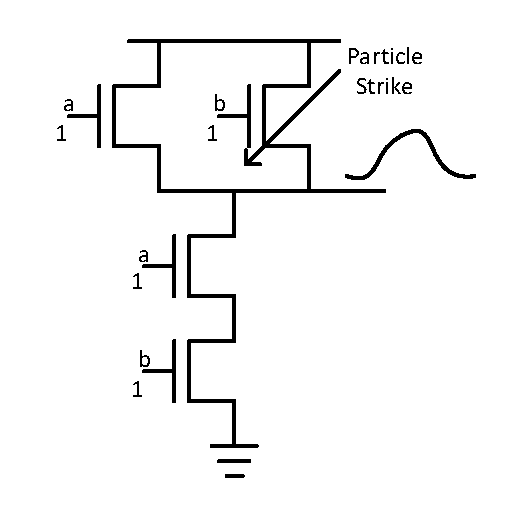
\includegraphics[width=0.55\linewidth]{Figures/NAND_Strike}
	%where an .eps filename suffix will be assumed under latex, 
	%and a .pdf suffix will be assumed for pdflatex; or what has been declared
	%via \DeclareGraphicsExtensions.
	\caption{A low-high-low transient pulse being generated by a strike on the PMOS.}
	\label{NANDS}
\end{figure}

\begin{table}[h]
	\begin{center}
		\caption{Functions for Transient Pulse Generation}
		\label{table:gentable}
		\begin{tabular}{|c|c|c|}
			\hline
			Gate & Polarity & Generation Function ($F(G)$) \\ 
			\hline
			AND & Rising & $F(G) =  \lnot (I_1 \land I_2 \land ... I_N)$ \\
			\hline
			AND & Falling & $F(G) = I_1 \land I_2 \land ... I_N$ \\
			\hline
			NAND & Rising & $F(G) = I_1 \land I_2 \land ... I_N$ \\
			\hline
			NAND & Falling & $F(G) = \lnot (I_1 \land I_2 \land ... I_N)$ \\
			\hline
			OR & Rising & $F(G) = \bar{I_1} \land \bar{I_2} \land ... \bar{I_N}$ \\
			\hline
			OR & Falling & $F(G) = \lnot ( \bar{I_1} \land \bar{I_2} \land ... \bar{I_N})$ \\
			\hline
			NOR & Rising & $F(G) = \lnot ( \bar{I_1} \land \bar{I_2} \land ... \bar{I_N})$ \\
			\hline
			NOR & Falling & $F(G) = \bar{I_1} \land \bar{I_2} \land ... \bar{I_N}$ \\
			\hline
		\end{tabular}
	\end{center}
\end{table}

For the consideration of the generation of METs, the above equations must be modified such that the joint probability of the error occurring is considered. In the case of pulse generation, it is assumed that a single radiation particle will strike two or more gates causing transient pulses. As stated previously, in order for a pulse with a specific polarity to be generated, the output of the gate must have a specific value. Based on this, the probability of pulses being generated ($P_{gen}$) assuming strikes $N$ gates with sufficient energy is given in equation \ref{pul_gen} where $P(G_{i,p})$ is the probability that gate $G_i$ is capable of generating a pulse of polarity $p$. If the pulse generated is rising, $G_{i,p}$ pertains to the probability that the output of $G_{i,p}$ is "0". If the pulse is falling, $G_{i,p}$ is the probability of the output being "1".

\begin{equation} \label{pul_gen}
P_{gen} = \prod_{i=1}^{N} P(G_{i, p})
\end{equation}

A particle hitting two transistors simultaneously allows for multiple cases since the input may be such that the struck gate is not blocking. Based on this, the total number of possible ways a strike can produce a pulse ($P_{num}$) is given in equation \ref{num_eq} assuming a $N$ number of struck gates and $r$ as the number of gates that produce a transient pulse.

\begin{equation} \label{num_eq}
P_{num} = 2*\sum_{r=1}^{N} \frac{N!}{(N-r)!}
\end{equation}

Equation \ref{num_eq} is based on the fact that multiple pulses are not always generated when a particle strikes both transistors. As stated previously, the polarity and existence of the pulse depends on the input patterns. If one assumes that the particle hits a $N$ number of gates, this creates a $P_{num}$ number of cases where $P(C_i)$ represents the probability of case $i$ calculated using equation \ref{pul_gen}. The total probability of the inputs having the values to generate a SET or MET $P_{gen}$ is given below:

\begin{equation} \label{err_eq}
P_{gen} = \sum_{i=1}^{P_{num}} P(C_i)
\end{equation}

In the case of a pulse being propagated to the input of gate, the pulse will be masked if one of the off-inputs has a controlling value. Fig. \ref{Prop_NAND} gives a NAND gate with one of the inputs having a pulse and the other input having a controlling "0" value. In this case, the output will be a logical "1" value despite the pulse on the input.

\begin{figure}[!htbp]
	\centering
	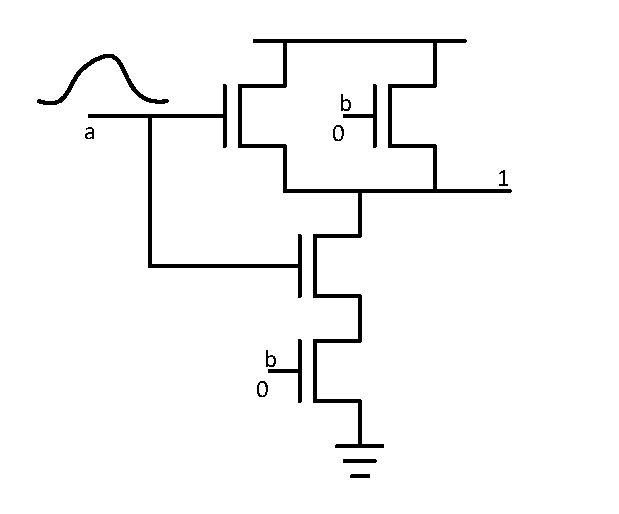
\includegraphics[width=0.55\linewidth]{Figures/Prop_func}
	%where an .eps filename suffix will be assumed under latex, 
	%and a .pdf suffix will be assumed for pdflatex; or what has been declared
	%via \DeclareGraphicsExtensions.
	\caption{A transient pulse being masking by a controlling value on the off-input.}
	\label{Prop_NAND}
\end{figure}

To calculate the logical masking factor during pulse propagation, the functions of the off-inputs are calculated using the logical AND operation. Assume that $F(OI_i)$ is the Boolean function of the off-input $OI_i$ representing the input patterns that allow a non-controlling value and there are a $N$ number of inputs, the function representing the case where the pulse is propagated $F(M)$ is given below:

\begin{equation} \label{prop_eq}
F(M) = F(OI_1) \land F(OI_2) \land ... F(OI_N)
\end{equation}

In equation \ref{prop_eq} only $N-1$ inputs are considered since the input which contains the transient pulse is not included in the calculation. 

For the consideration of METs, two or more pulses may arrive at a gate. If the two pulse case is assumed, there are 3 possible ways that the pulses can be propagated: the pulse on $a$ is propagated and $b$ is masked, the pulse on $b$ is propagated and $a$ is masked and, lastly, the both pulses are propagated simultaneously providing an output pulse. Fig. \ref{Prop_MET} provides an illustration of the cases.

\begin{figure}[!htbp]
	\centering
	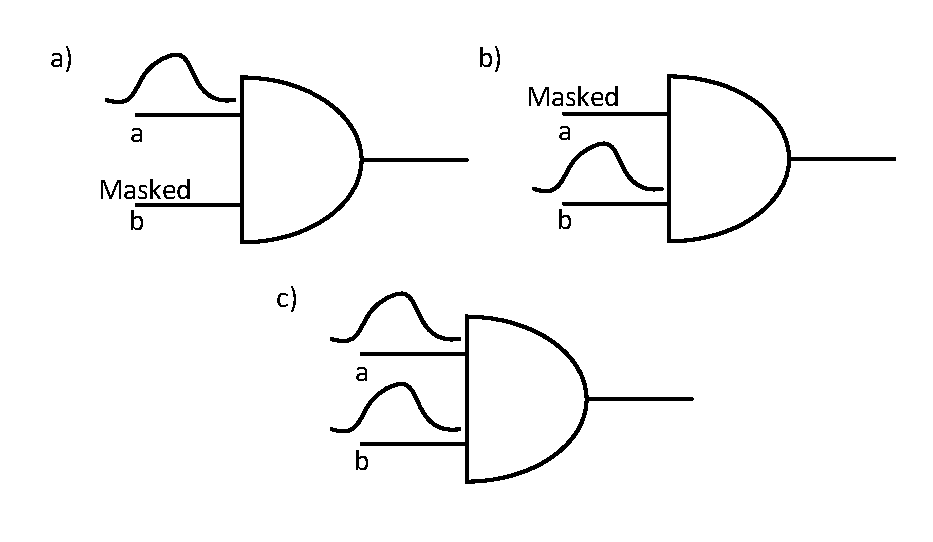
\includegraphics[width=0.80\linewidth]{Figures/Prop_MET}
	%where an .eps filename suffix will be assumed under latex, 
	%and a .pdf suffix will be assumed for pdflatex; or what has been declared
	%via \DeclareGraphicsExtensions.
	\caption{(a) A transient pulse arriving on input a and masked on b. (b) A pulse arriving on input b and masked on a. (c) Two pulses arriving on the inputs simultaneously.}
	\label{Prop_MET}
\end{figure}

Table \ref{table:prop_table} gives the propagation functions $F(G)$ for each case with $F(a_p)$ and $F(b_p)$ being the functions representing the input values that allow for the pulse to be propagated to inputs a and b respectively. While this example is only for a two input gate, multiple input gates can be considered similarly.

\begin{table}[h]
	\begin{center}
		\caption{Functions for Transient Pulse Generation}
		\label{table:prop_table}
		\begin{tabular}{|c|c|}
			\hline
			Case & Propagation Function ($F(G)$) \\ 
			\hline
			a & $F(G) = F(a_p) \land \lnot F(b_p)$ \\
			\hline
			b & $F(G) = \lnot F(a_p) \land F(b_p)$ \\
			\hline
			c & $F(G) = F(a_p) \land F(b_p)$ \\
			\hline
		\end{tabular}
	\end{center}
\end{table}

Based off equation \ref{num_eq}, the total number of cases can be calculated as the number of combinations assuming $i = 1,2,...N$ simultaneous pulses. Assuming that $P_{num}$ is the number of possible cases and $r_i$ represents a $i$ number of concurrent pulses, the equation for the total number of propagation cases is given below:

\begin{equation} \label{prop_num}
P_{num} = \sum_{i=1}^{N} \frac{N!}{(N-r_i)!}
\end{equation} 

Based on equation \ref{prop_num}, the total probability of multiple convergent pulses at a gate $G$ ($P(G_{tot})$) with the assumption that $P(G_i)$ is the probability of case $i$ on gate $G$ is given below:

\begin{equation} \label{tot_gate}
P(G_{tot}) = \sum_{i}^{P_{num}} P(G_i)
\end{equation}

When a MET is generated, it is represented as an event $E_k$ with $k$ being the event number. For each event, the generated transients are propagated through gates to the primary outputs. Once the pulse arrive at the gate output, the temporal masking probability can be considered. Based off the equation found in \cite{Omana_Trap}, let  $P_{L,i}$ is the probability of the pulse being latch on gate $i$, $W$ be the pulse width, $t_{setutp}$ and $t_{hold}$ being the setup and hold times respectively and $T_{clk}$ be the clock period, the probability of a pulse being latch on an output flip-flop is calculated in the below equation:

\begin{equation} \label{temp_eq}
P_{L,i} = \frac{W - (t_{setup} + t_{hold})}{T_{clk}}
\end{equation}

Assuming that the pulses from event $E_k$ propagate to a $M$ number of primary outputs with each gate having a probability of $P_{L,i}$ calculated as in equation \ref{temp_eq}, the probability of error for event $E_k$ is calculated as the following:  

\begin{equation} \label{event_eq}
P(E_k) = \sum_{i=1}^{M} P_{L,i}
\end{equation}

To evaluate the error probability for all events, the mean error susceptibility (MES), defined in \cite{METSys} is used. The MES represents the average probability of error for all events combined. Assuming that there are a $n_E$ number of events, $n_d$ number of input probability distributions and that $K$ is the number of injected events, the MES is found using the following equation:

\begin{equation} \label{MES}
MES = \sum_{k=1}^{K} \frac{P(E_k)}{n_E n_d}
\end{equation}

Based off the MES, the soft error rate ($SER$) can be calculated as in below where $R_{eff}$ represents the effective concentration of particle in the given area, $P_{eff}$ is the probability of a particle hitting the sensitive region of a transistor and $A$ as the area of the sensitive volumes.

\begin{equation} \label{SER}
SER = MES*R_{eff}*P_{eff}*A 
\end{equation}

\section{Description of the FAST\_MET Simulator}

FAST\_MET is a fast and accurate tool to estimate the soft error rate. The method aims to provide a good trade-off between simulation time and accurate SER calculation. To accurately determine the logical masking effects, BDDs are used. A BDD is a tree structure which can be used to represent a Boolean function. The first instance of the use of BDDs for function representation was proposed in \cite{Bryant1986} and has continued to be used regularly in circuit simulation and synthesis since. Fig. \ref{BDD_AND} gives the representation of a AND gate as BDD. Note that the structure consists of nodes which represent variables. For each node, there are two branches, one denoting a "true" value and the other a "false" value. The BDD graph also consists of multiple paths to two terminating nodes, one with a "true" value denoted by "1" and one with a "false" value denoted by "0".

\begin{figure}[!htbp]
	\centering
	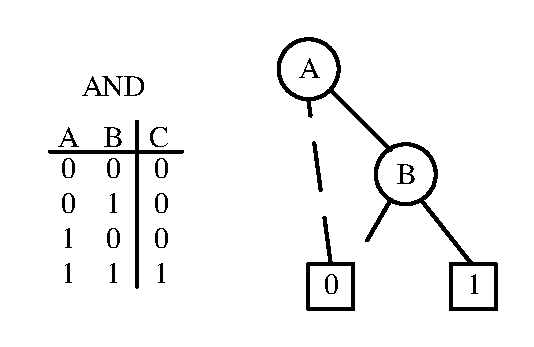
\includegraphics[width=0.65\linewidth]{Figures/BDDFunc}
	%where an .eps filename suffix will be assumed under latex, 
	%and a .pdf suffix will be assumed for pdflatex; or what has been declared
	%via \DeclareGraphicsExtensions.
	\caption{The truth table and corresponding BDD for an AND gate.}
	\label{BDD_AND}
\end{figure}

	The main advantage of a BDD is that they provide an efficient canonical form to represent a Boolean function. Specifically, this means that Boolean operations (such as AND, NAND, OR ... etc) can be easily and quickly applied to the graph. In the case of the FAST\_MET simulator, BDD representation of the functions are used to both calculate the signal probability and the probability for pulse propagation.

In FAST\_MET, the goal is to accurately and efficiently represent a sensitization function as a BDD. A sensitization function is defined as the Boolean function that allows for a generated transient pulse to propagate through a circuit. In other words, a sensitization is the function that represents all input patterns that sensitize the pulse to the output. 

The FAST\_MET simulator operates in a topological order. This implies that the primary inputs will be visited first. Once a primary input is visited, it is represented as a variable for in a BDD. Once all inputs are visited, the simulator starts on the gates within the circuit. When a gate is visited, the sensitization function representing the gate output is calculated. The "1" terminal on this BDD represents the Boolean function that makes the output a "1" value. To increase efficiency, the FAST\_MET simulator generates a rising and falling pulse at each gate using the method proposed in Chapter \ref{ch2} for a specific energy.

When a pulse is generated, the gate input functions are considered using the input sensitization functions. If the pulse is rising (starting from a low value then going high), the pulse is only generated when the output is low. To consider this, the BDD function is inverted such that a termination to "1" represents that case at which the pulse exists. Similarly, if the pulse is falling, the output must be a high value. Since the function already denotes a high value on the output, the sensitization function can be used directly. Additionally, as discussed in Section \ref{ch3:prelim}, in the case of a gate having multiple inputs, the output function must be considered according to Table \ref{table:gentable}. Using the table, the correct generation function can be found by applying the function for the gate specified. Fig. \ref{BDD_GEN} provides an example of the creation of the generation functions for a gate.

\begin{figure}[!htbp]
	\centering
	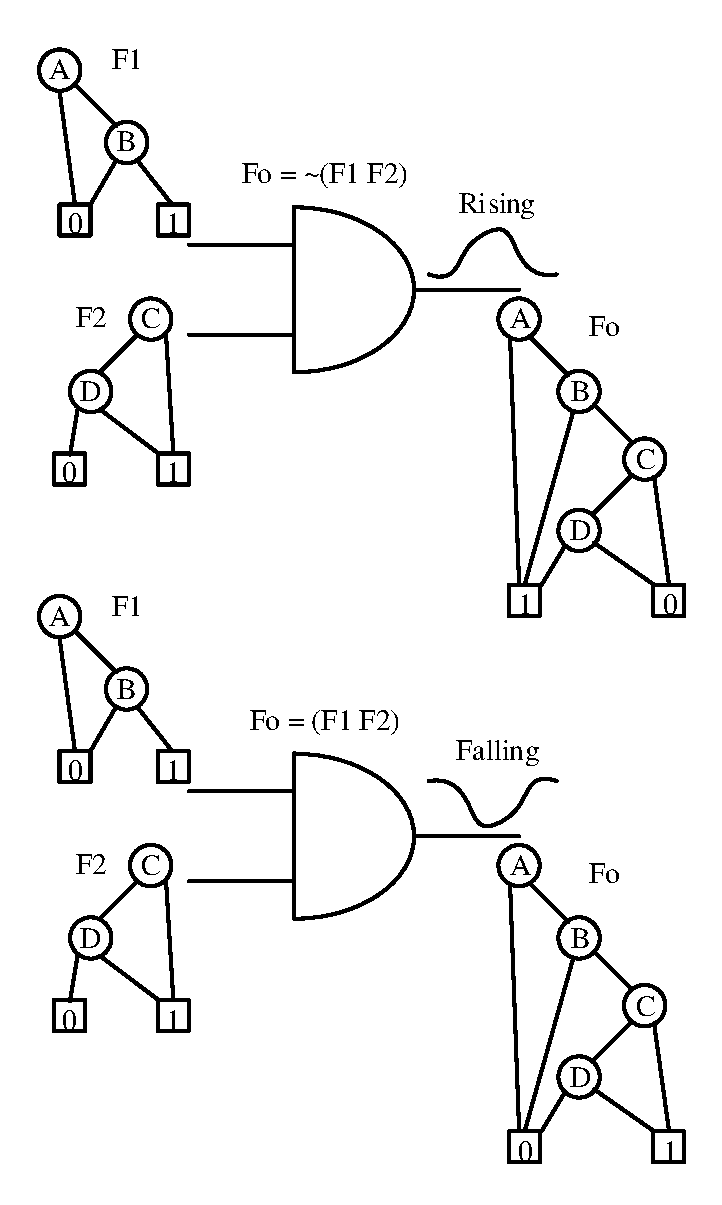
\includegraphics[width=0.65\linewidth]{Figures/gen_func}
	%where an .eps filename suffix will be assumed under latex, 
	%and a .pdf suffix will be assumed for pdflatex; or what has been declared
	%via \DeclareGraphicsExtensions.
	\caption{An example of the BDD creation for a rising and falling pulse,}
	\label{BDD_GEN}
\end{figure}

To consider the MET case, the location and correlation between the pulses must be considered. As discussed in \cite{Ebrahimi2016}, layout information is important in accurately modeling the location of the MET for a real design. Gates that are near each other in a netlist may not necessarily be close in the layout. In this section, for the sake of simplicity, METs are generated using close proximity nodes from the netlist. However, for the sake of simple comparison and analysis, using the netlist is not problematic. 